\subsection{26 августа. Пер. Кичкинекол Малый (1А)}
\textit{Метеоусловия: утром переменная облачность, днём, вечером сильный лождь, ветер.}

\begin{figure}[h!]
	\centering
	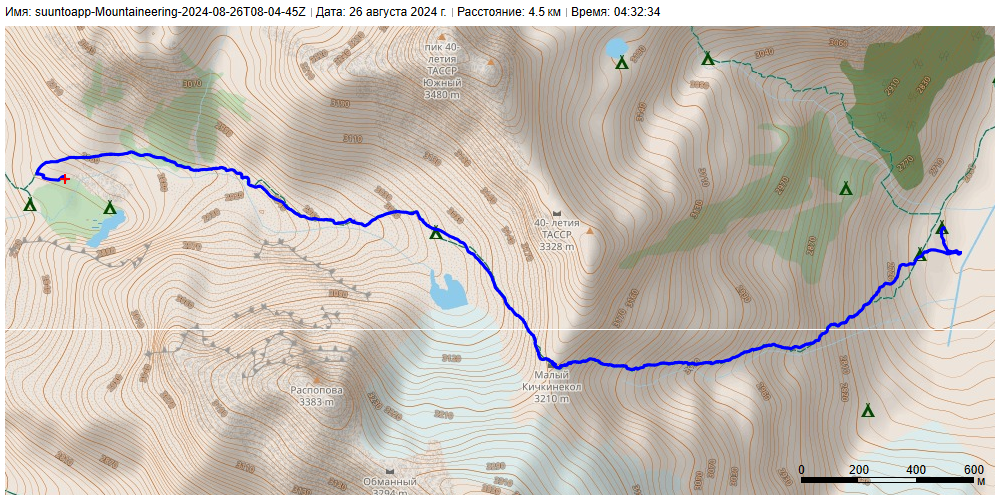
\includegraphics[angle=0, width=0.7\linewidth]{../pics/mini_maps/26}
	\label{fig:mini_26}
\end{figure}

Подъём в 08:00. Гроза закончилась, небо затянуто облаками, периодически выходит солнце. Выходим в 11:00, движемся по тропе, траверсирующей травянистый склон.  Тропа обходит водопад на западной оконечности поляны слева пхд. Встречаются туры, тропу видно хорошо. 
Постепенно травянистый склон переходит в морену.

\begin{figure}[h!]
	\centering
	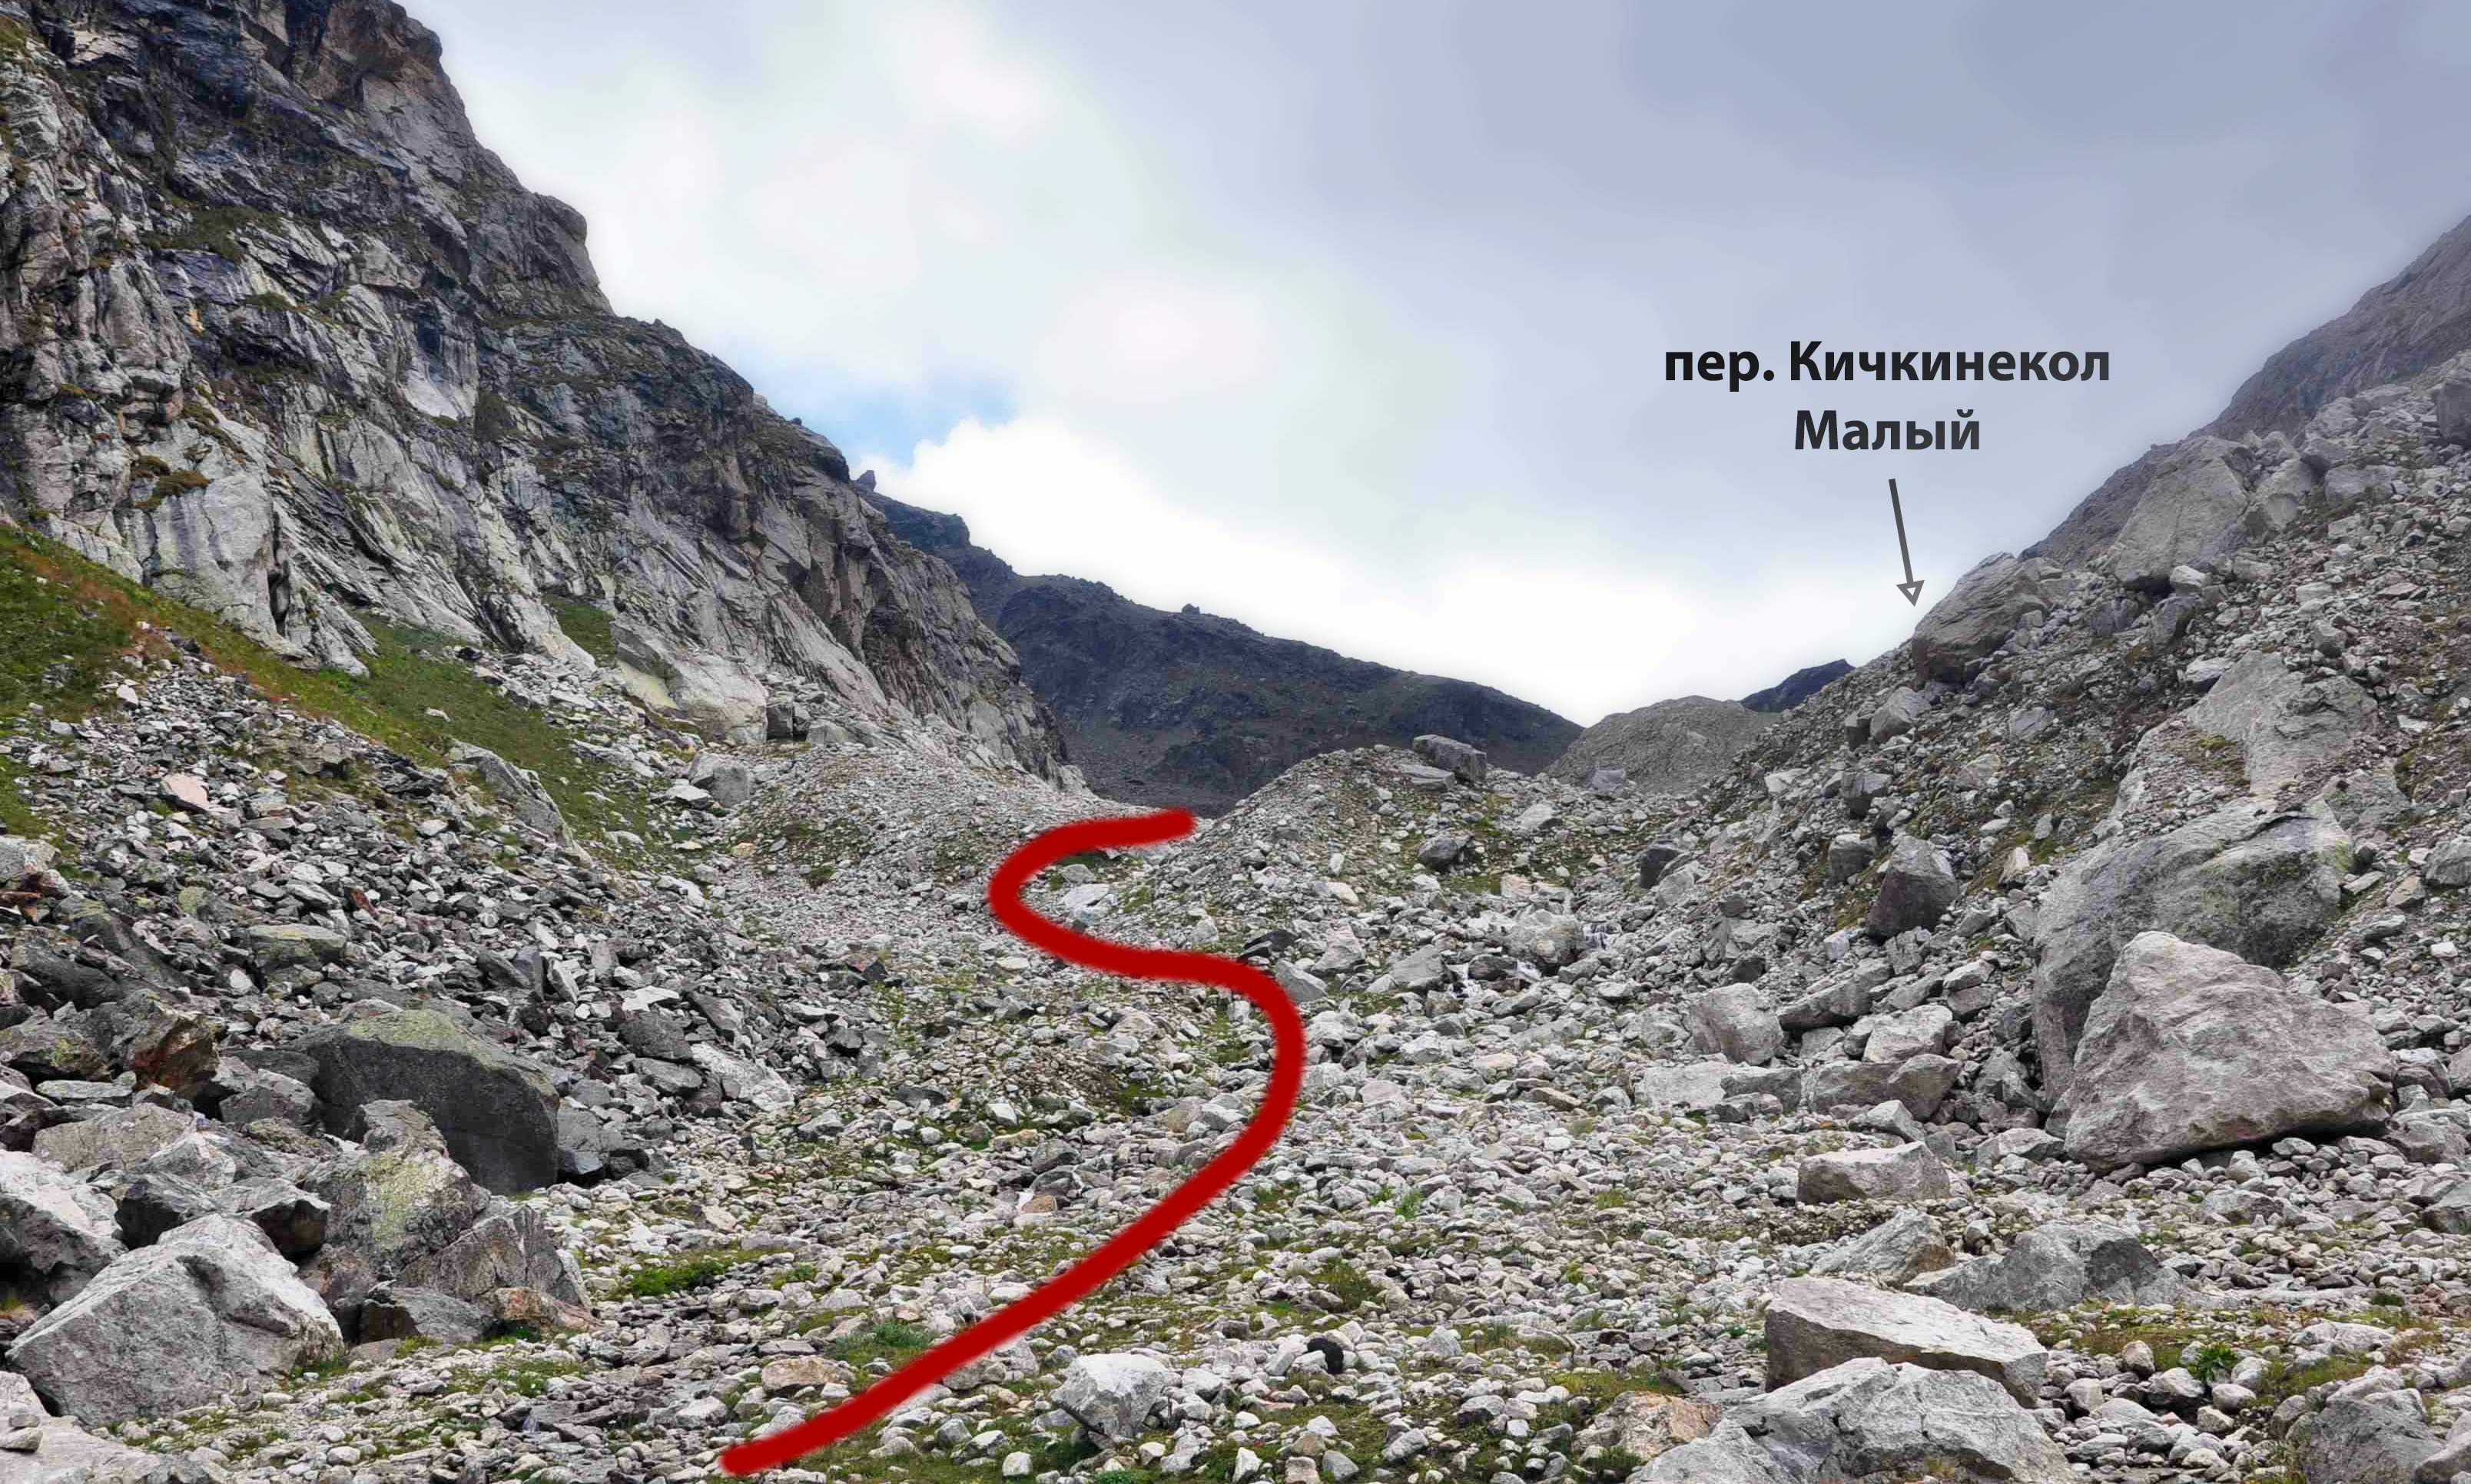
\includegraphics[width=0.7\linewidth]{../pics/DSC_0221.JPG}
	\caption{Путь подъёма на перевал}
	\label{fig:DSC_0221}
\end{figure}
 
 За поворотом нам открывается вид на наш перевал и цирк соседнего перевала Обманный (рис.~\ref{fig:DSC_0226},\ref{fig:DSC_0227}).
 
\begin{figure}[h!]
	\centering
	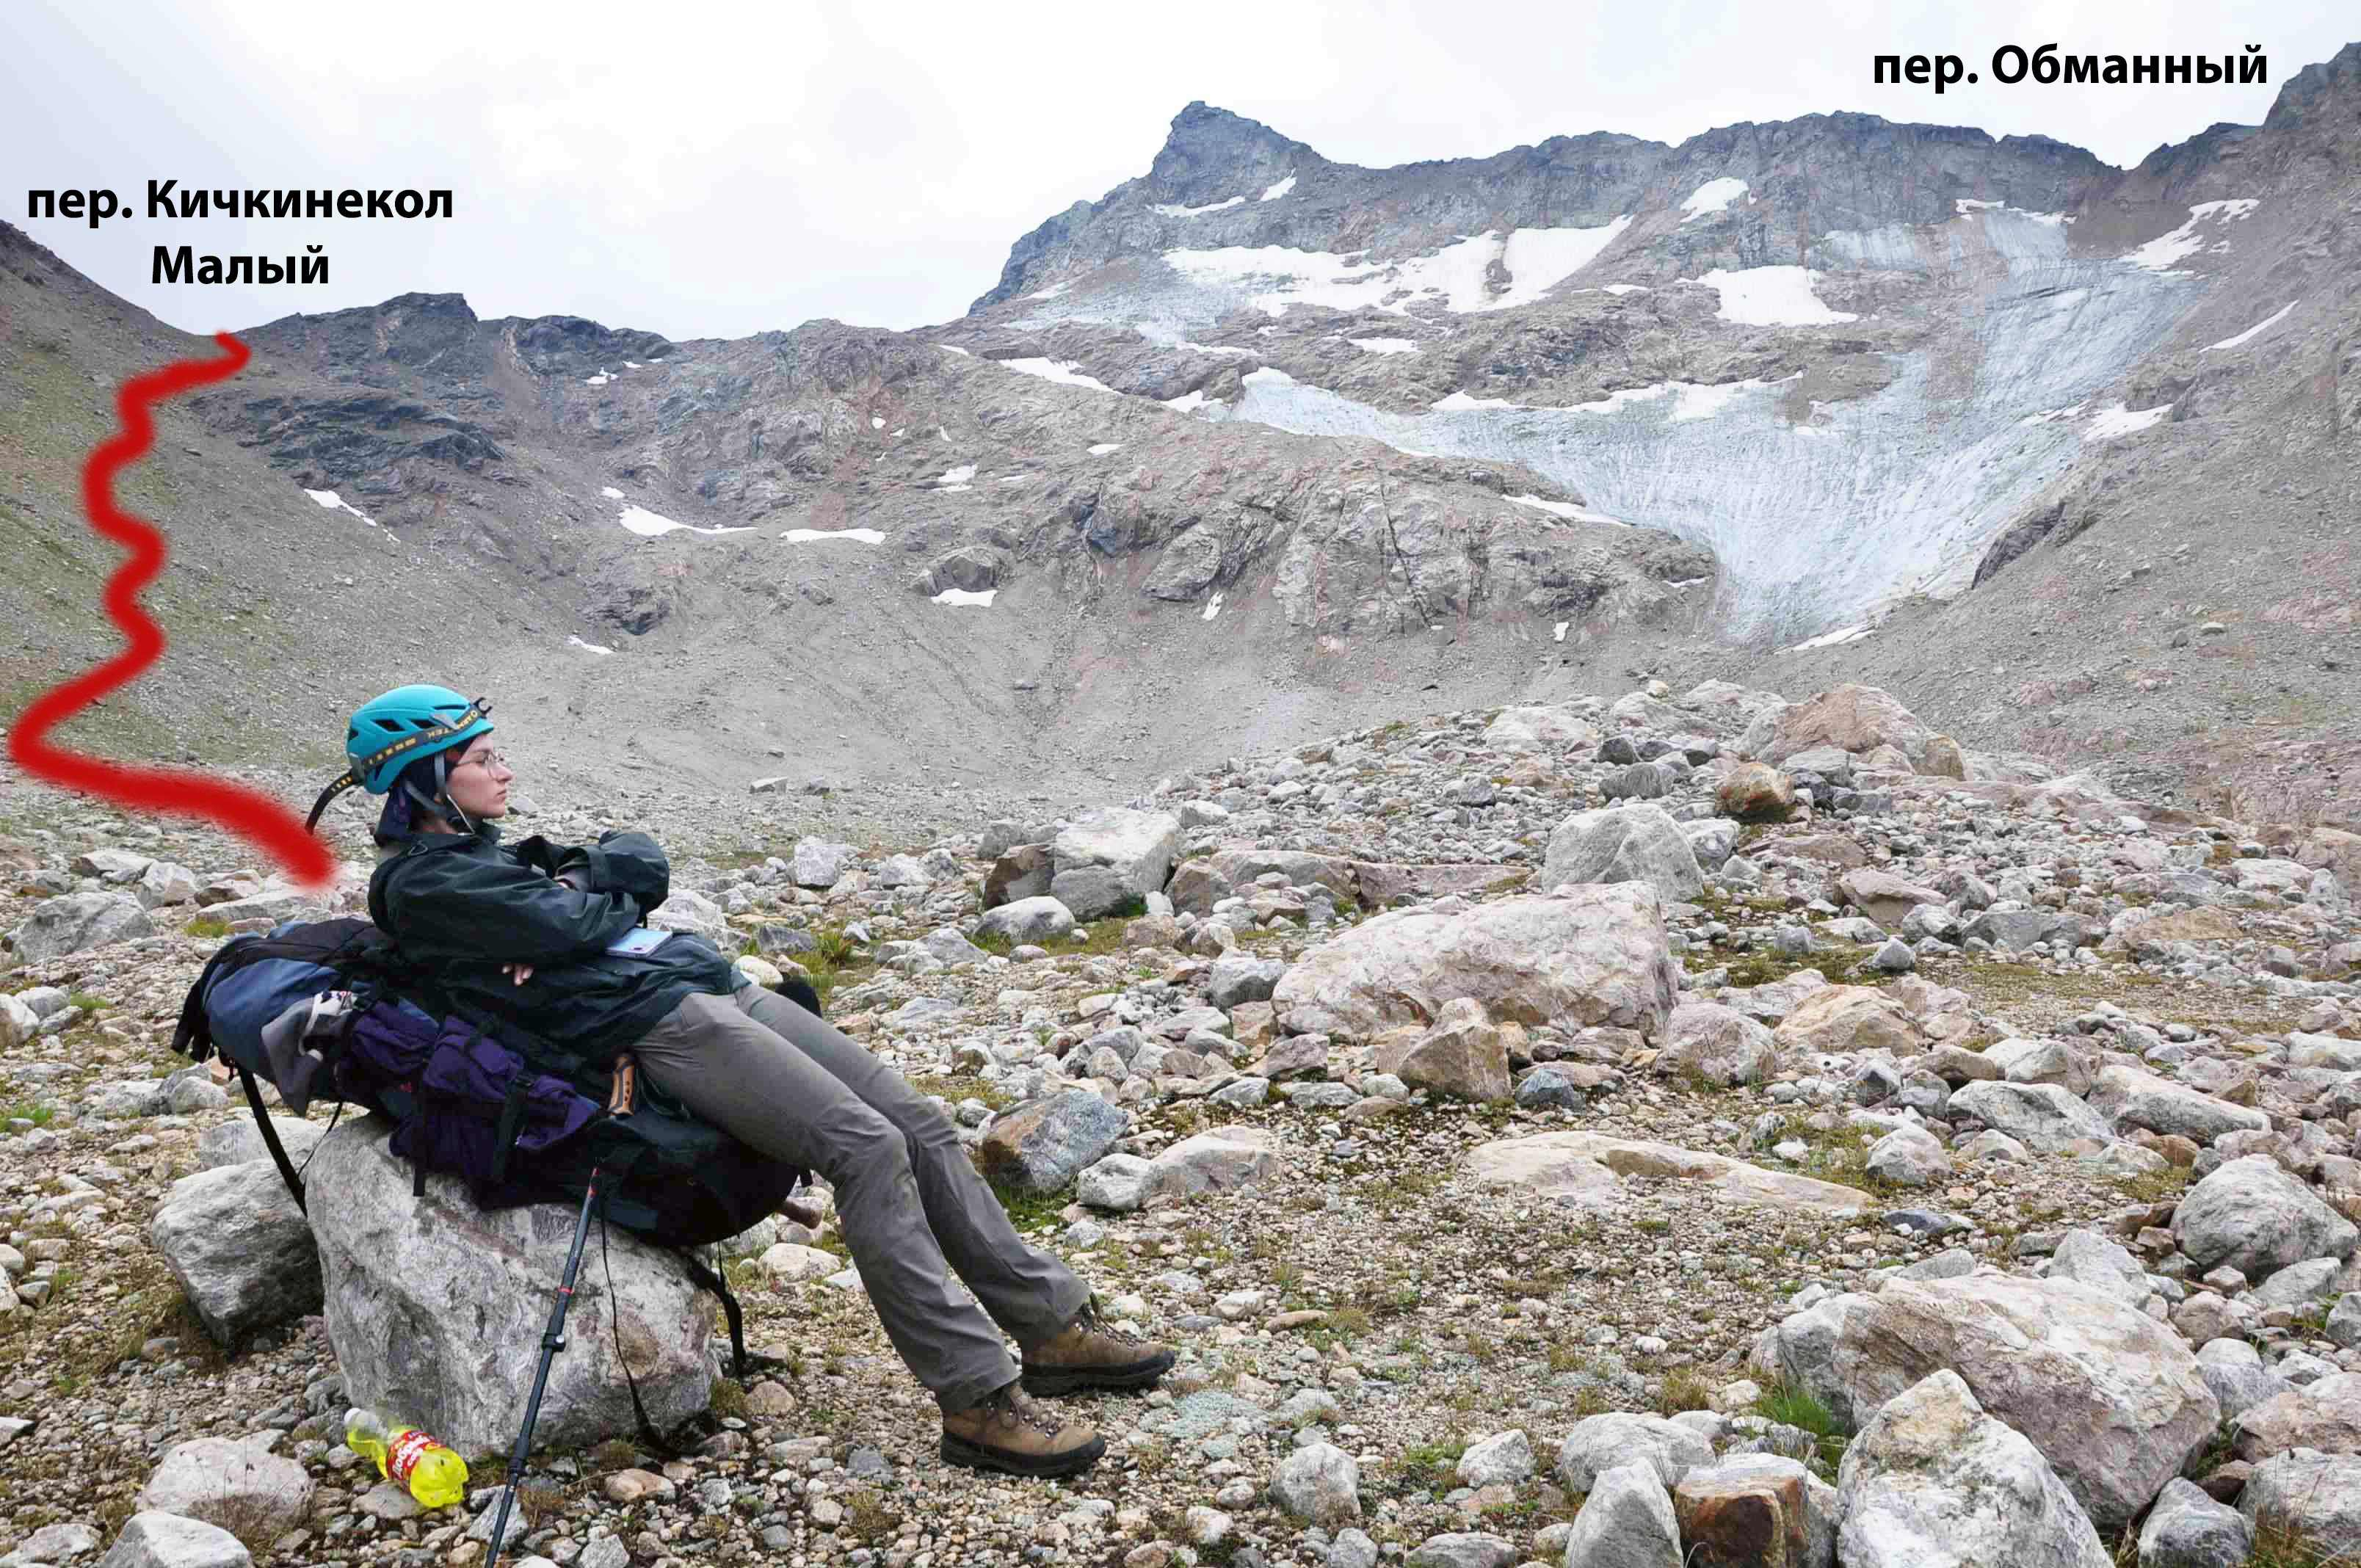
\includegraphics[width=0.7\linewidth]{../pics/DSC_0226}
	\caption{Маршрут движения группы}
	\label{fig:DSC_0226}
\end{figure}

Погода ухудшается, начинается небольшой дождь.


\begin{figure}[h!]
	\centering
	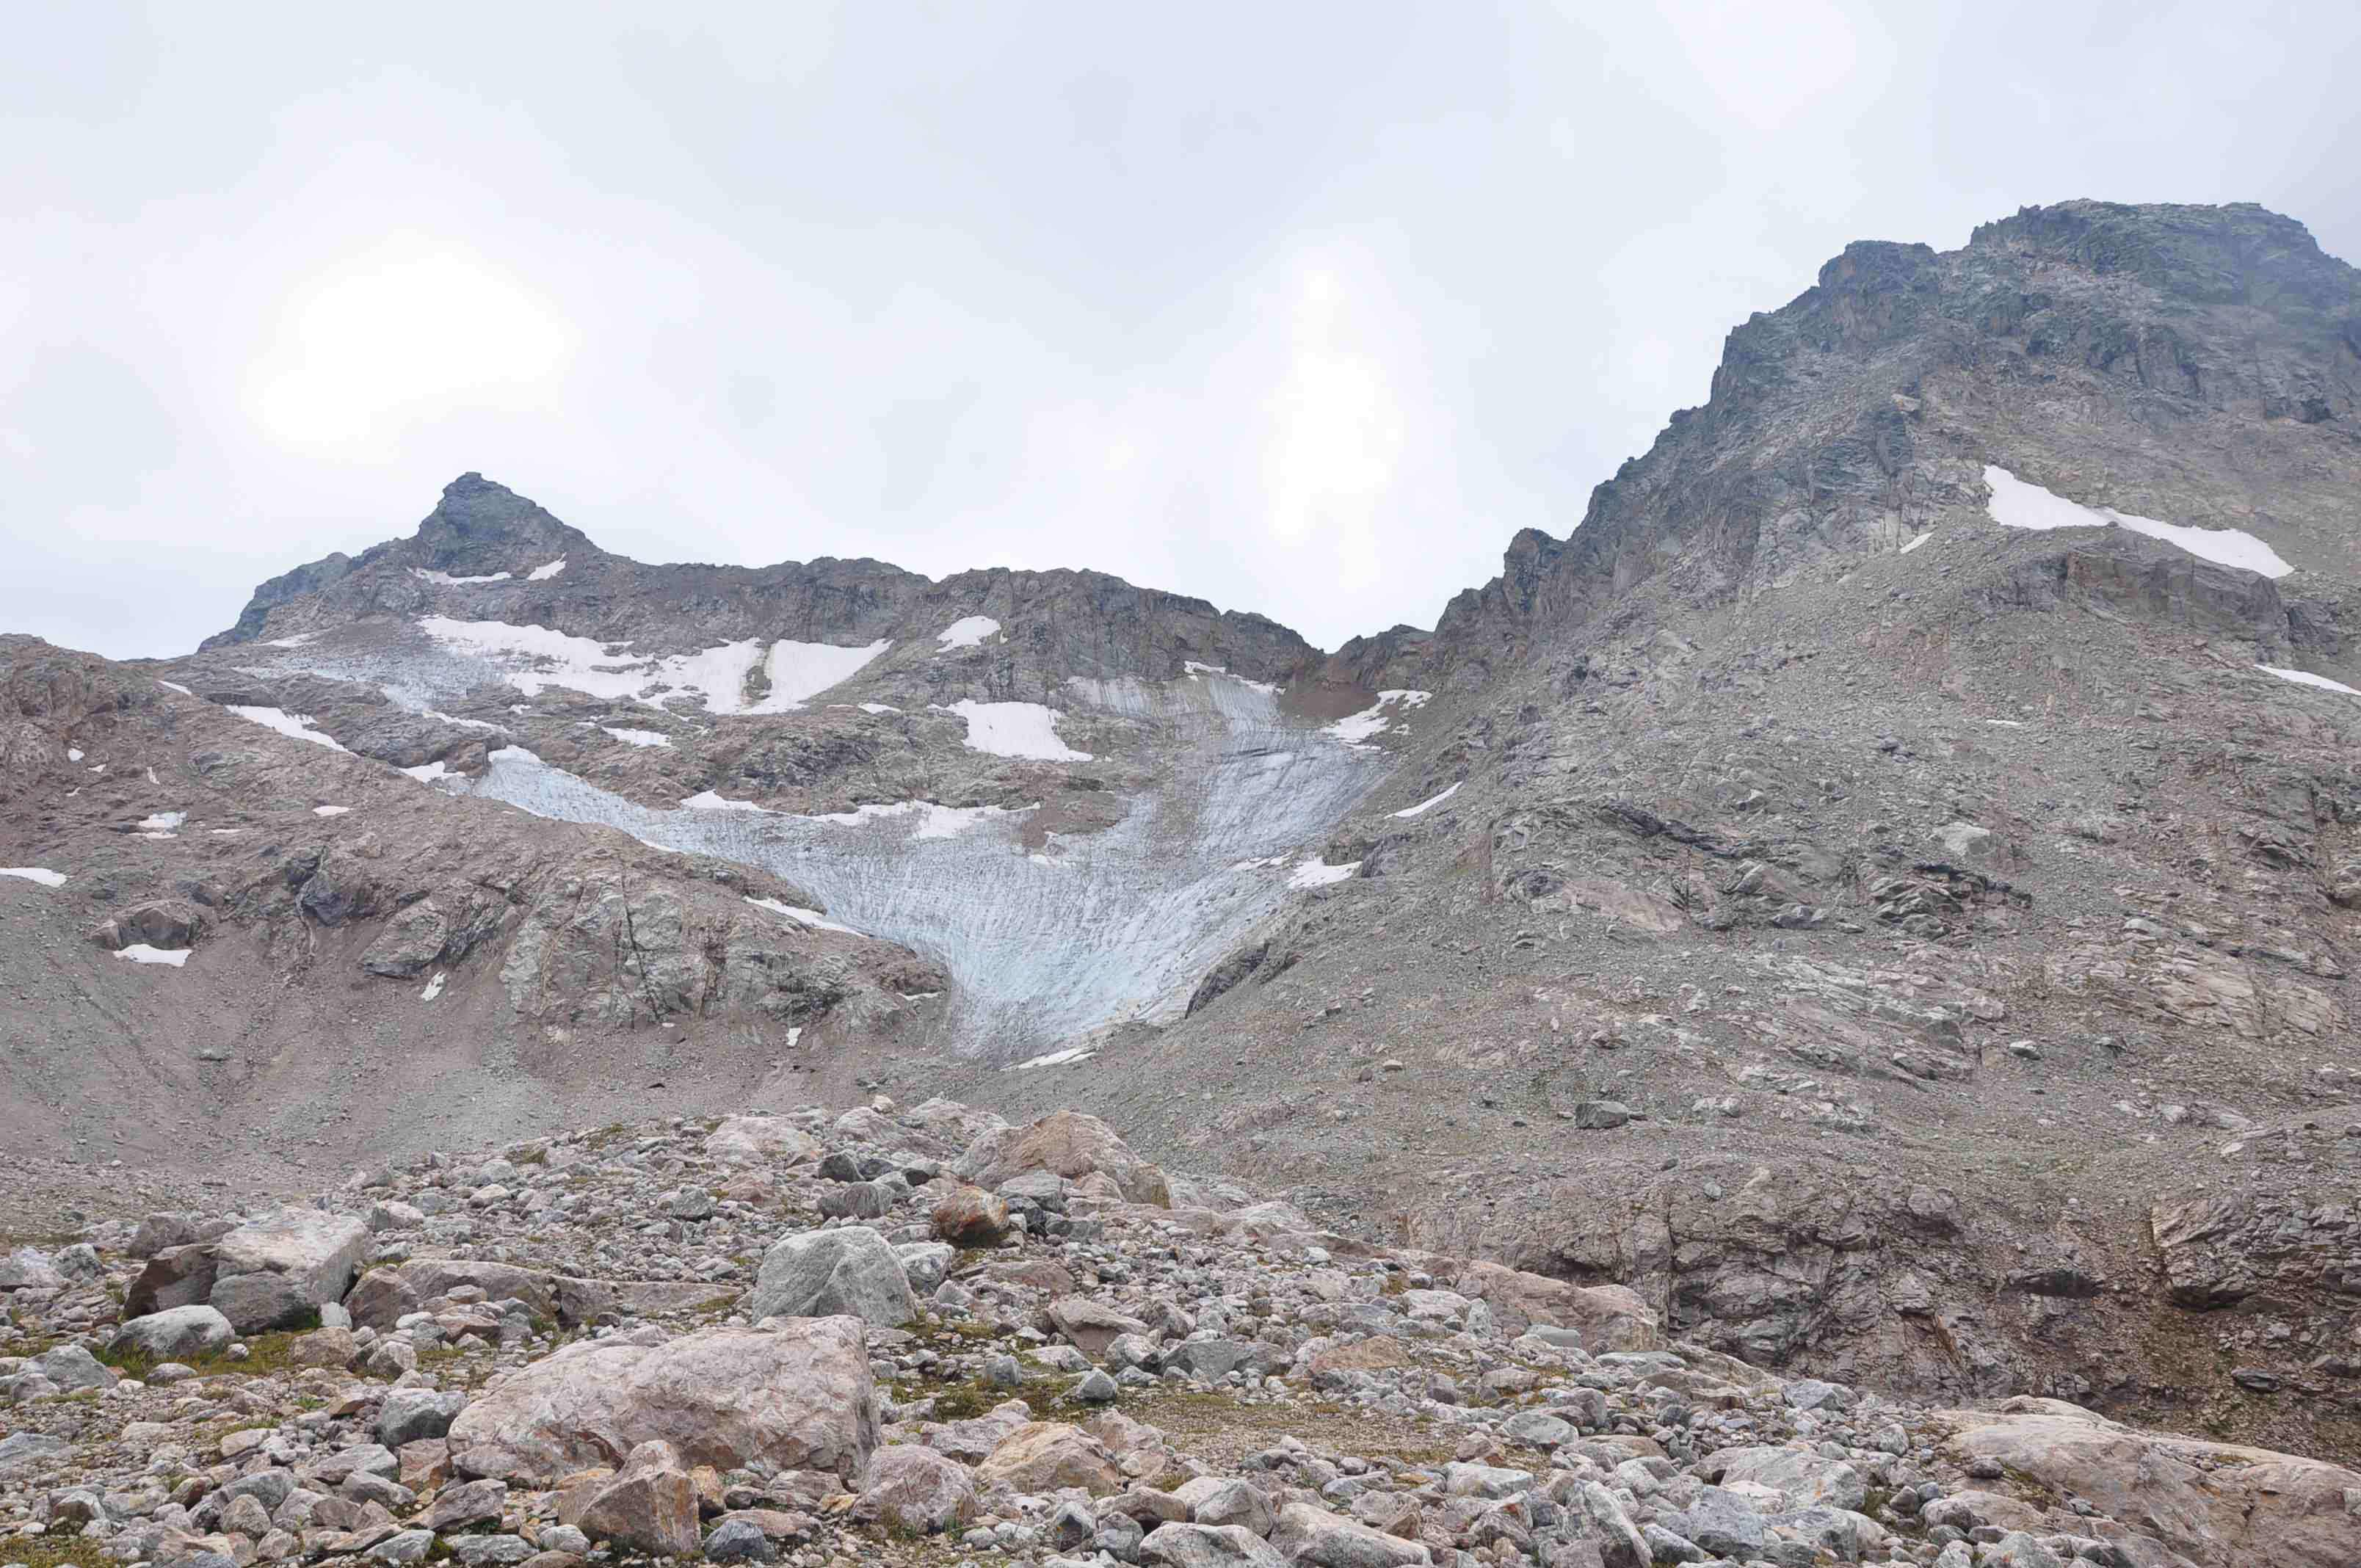
\includegraphics[width=0.7\linewidth]{../pics/DSC_0227.JPG}
	\caption{Цирк пер. Обманный справа пхд от пер. Кичкинекол Малый}
	\label{fig:DSC_0227}
\end{figure}


Подъём на перевал проходит по средней и мелкой осыпи, идём косыми траверсами с самостраховкой треккинговыми палками. Технической сложности не представляет.
В 13:15 заходим на перевал Кичкинекол Малый (рис.~\ref{fig:DSC_0239}). Погода совсем испортилась, идёт ливень с градом. Снимаем перевальную записку т/к <<Крокус>> (г.~Краснодар) от 24.08.2024~г., пишем свою, укрывая писаря от непогоды пончо, едим перевальный шоколад и в 13:22 начинаем спуск.


\begin{figure}[h!]
	\centering
	\begin{minipage}[h]{0.48\linewidth}
		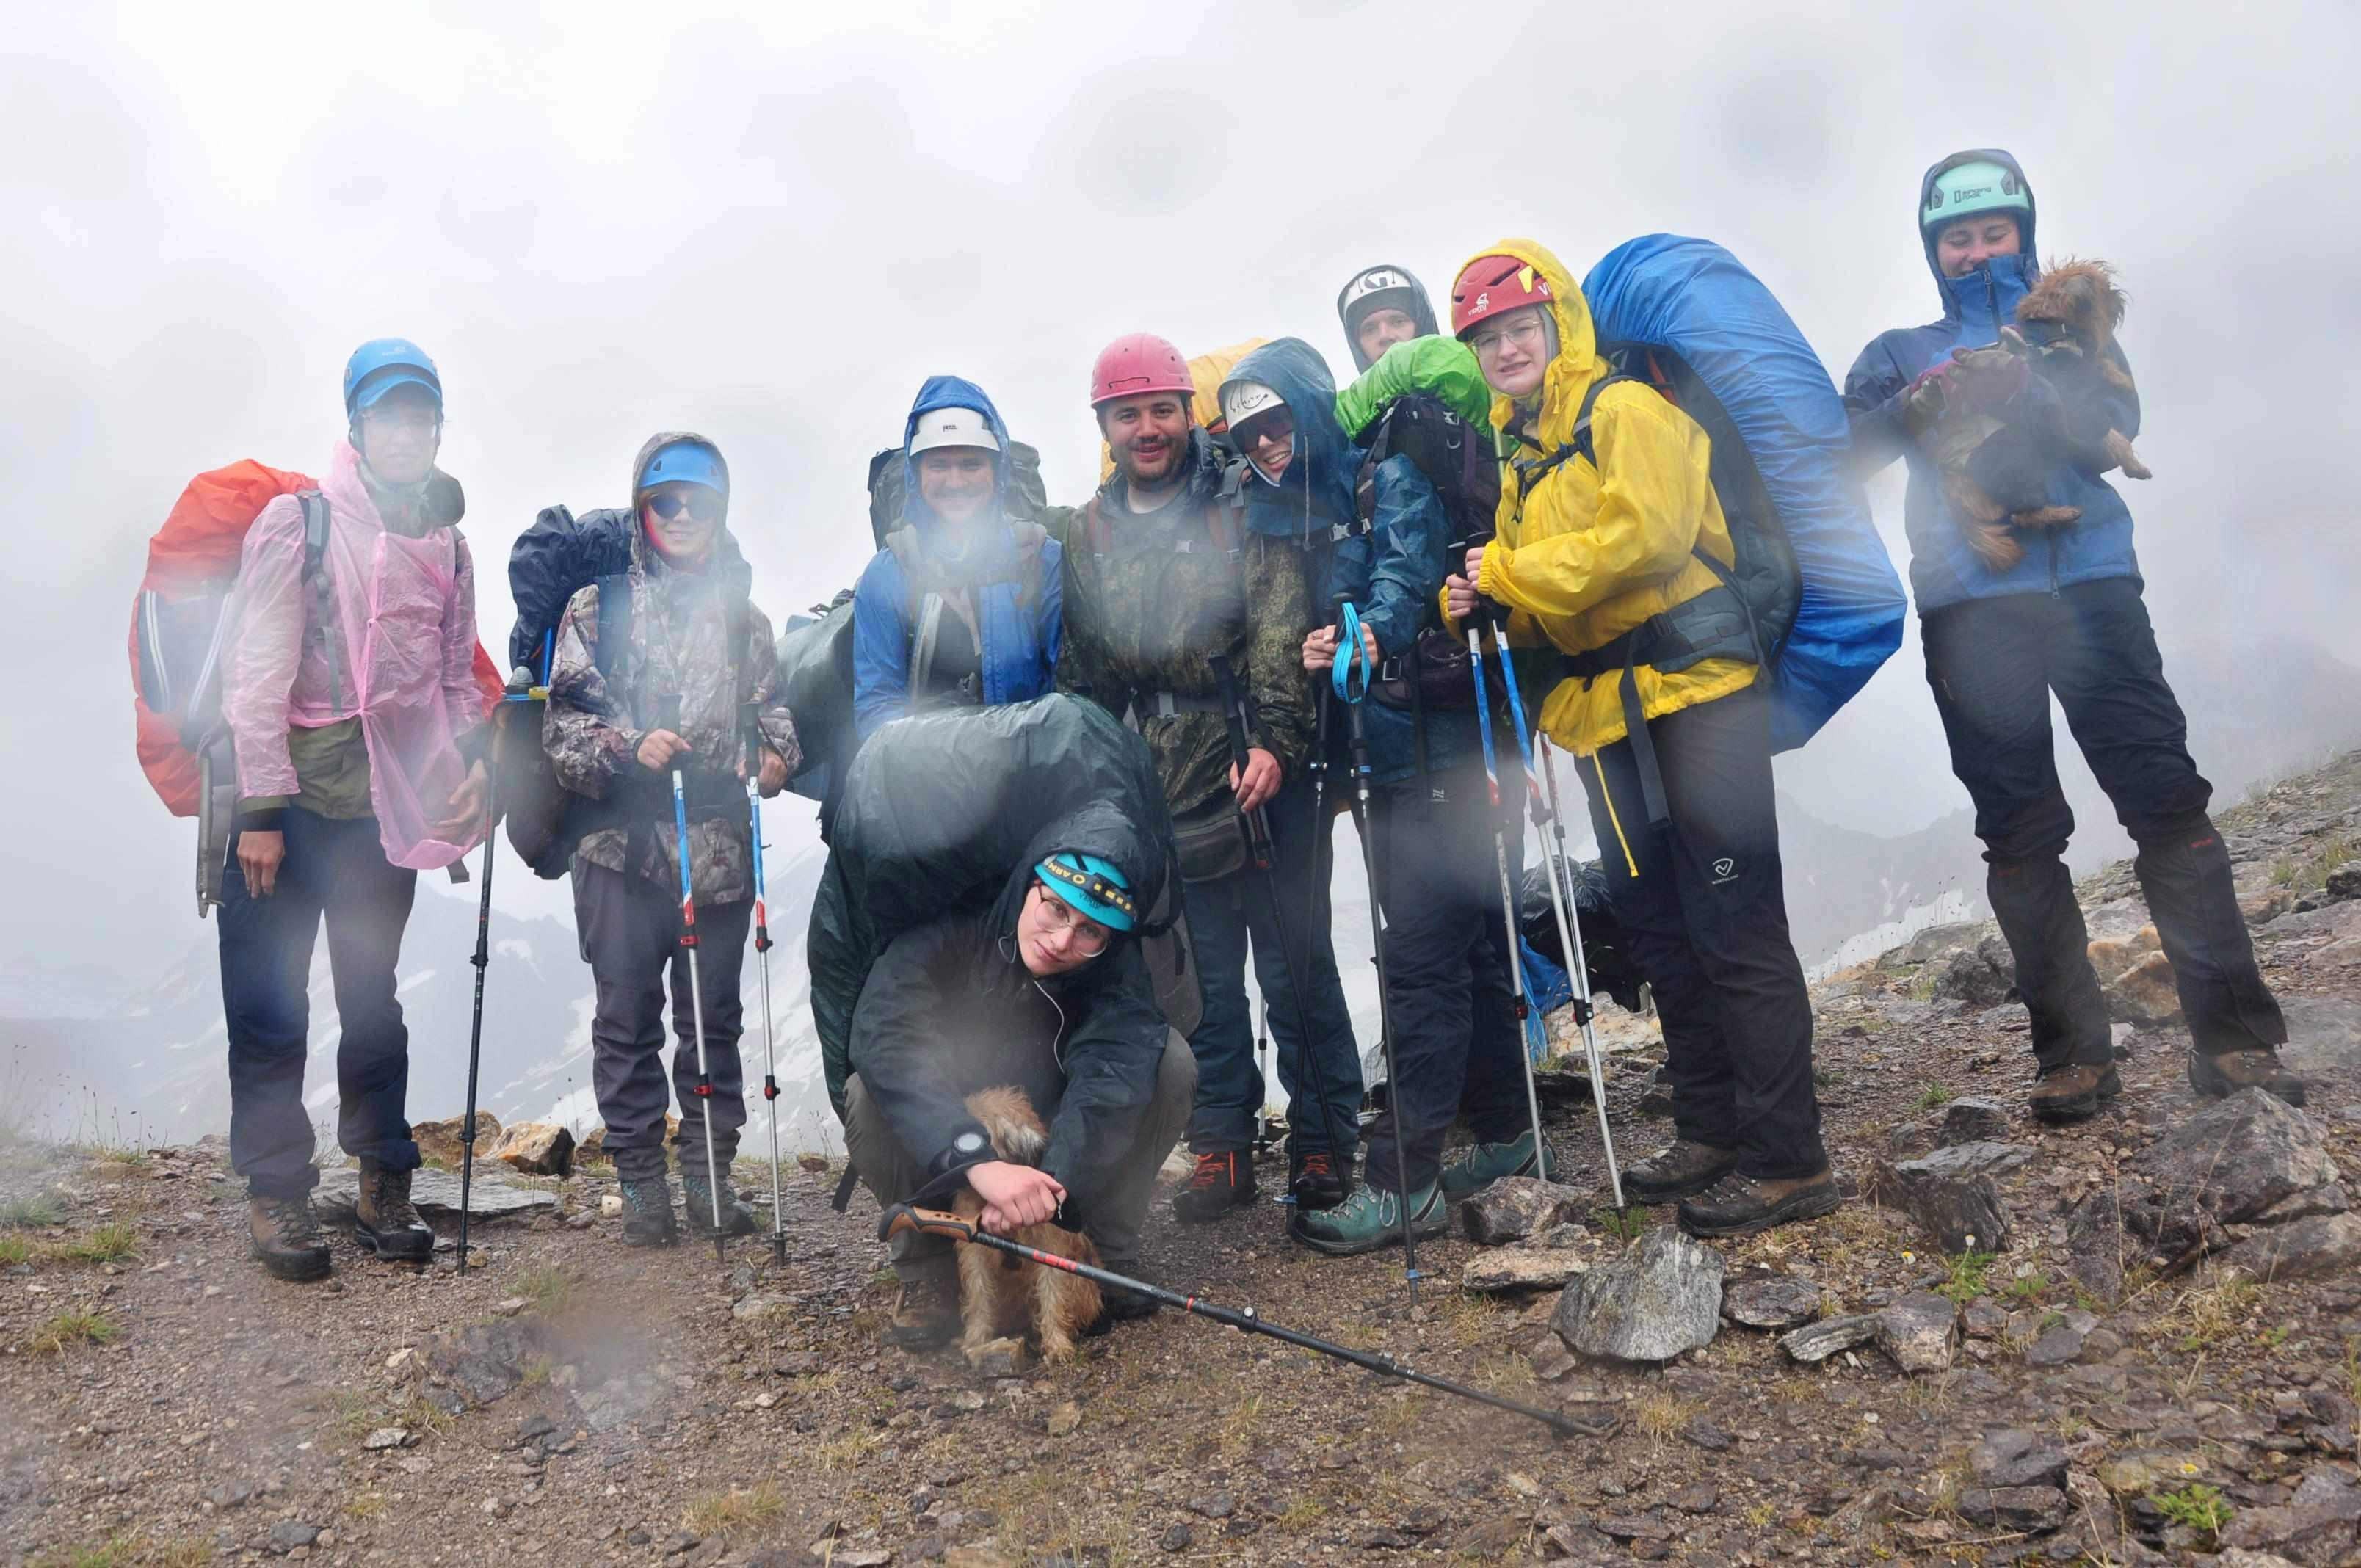
\includegraphics[width=0.99\linewidth]{../pics/DSC_0239.jpg}
	\end{minipage}
	\quad
	\begin{minipage}[h]{0.48\linewidth}
		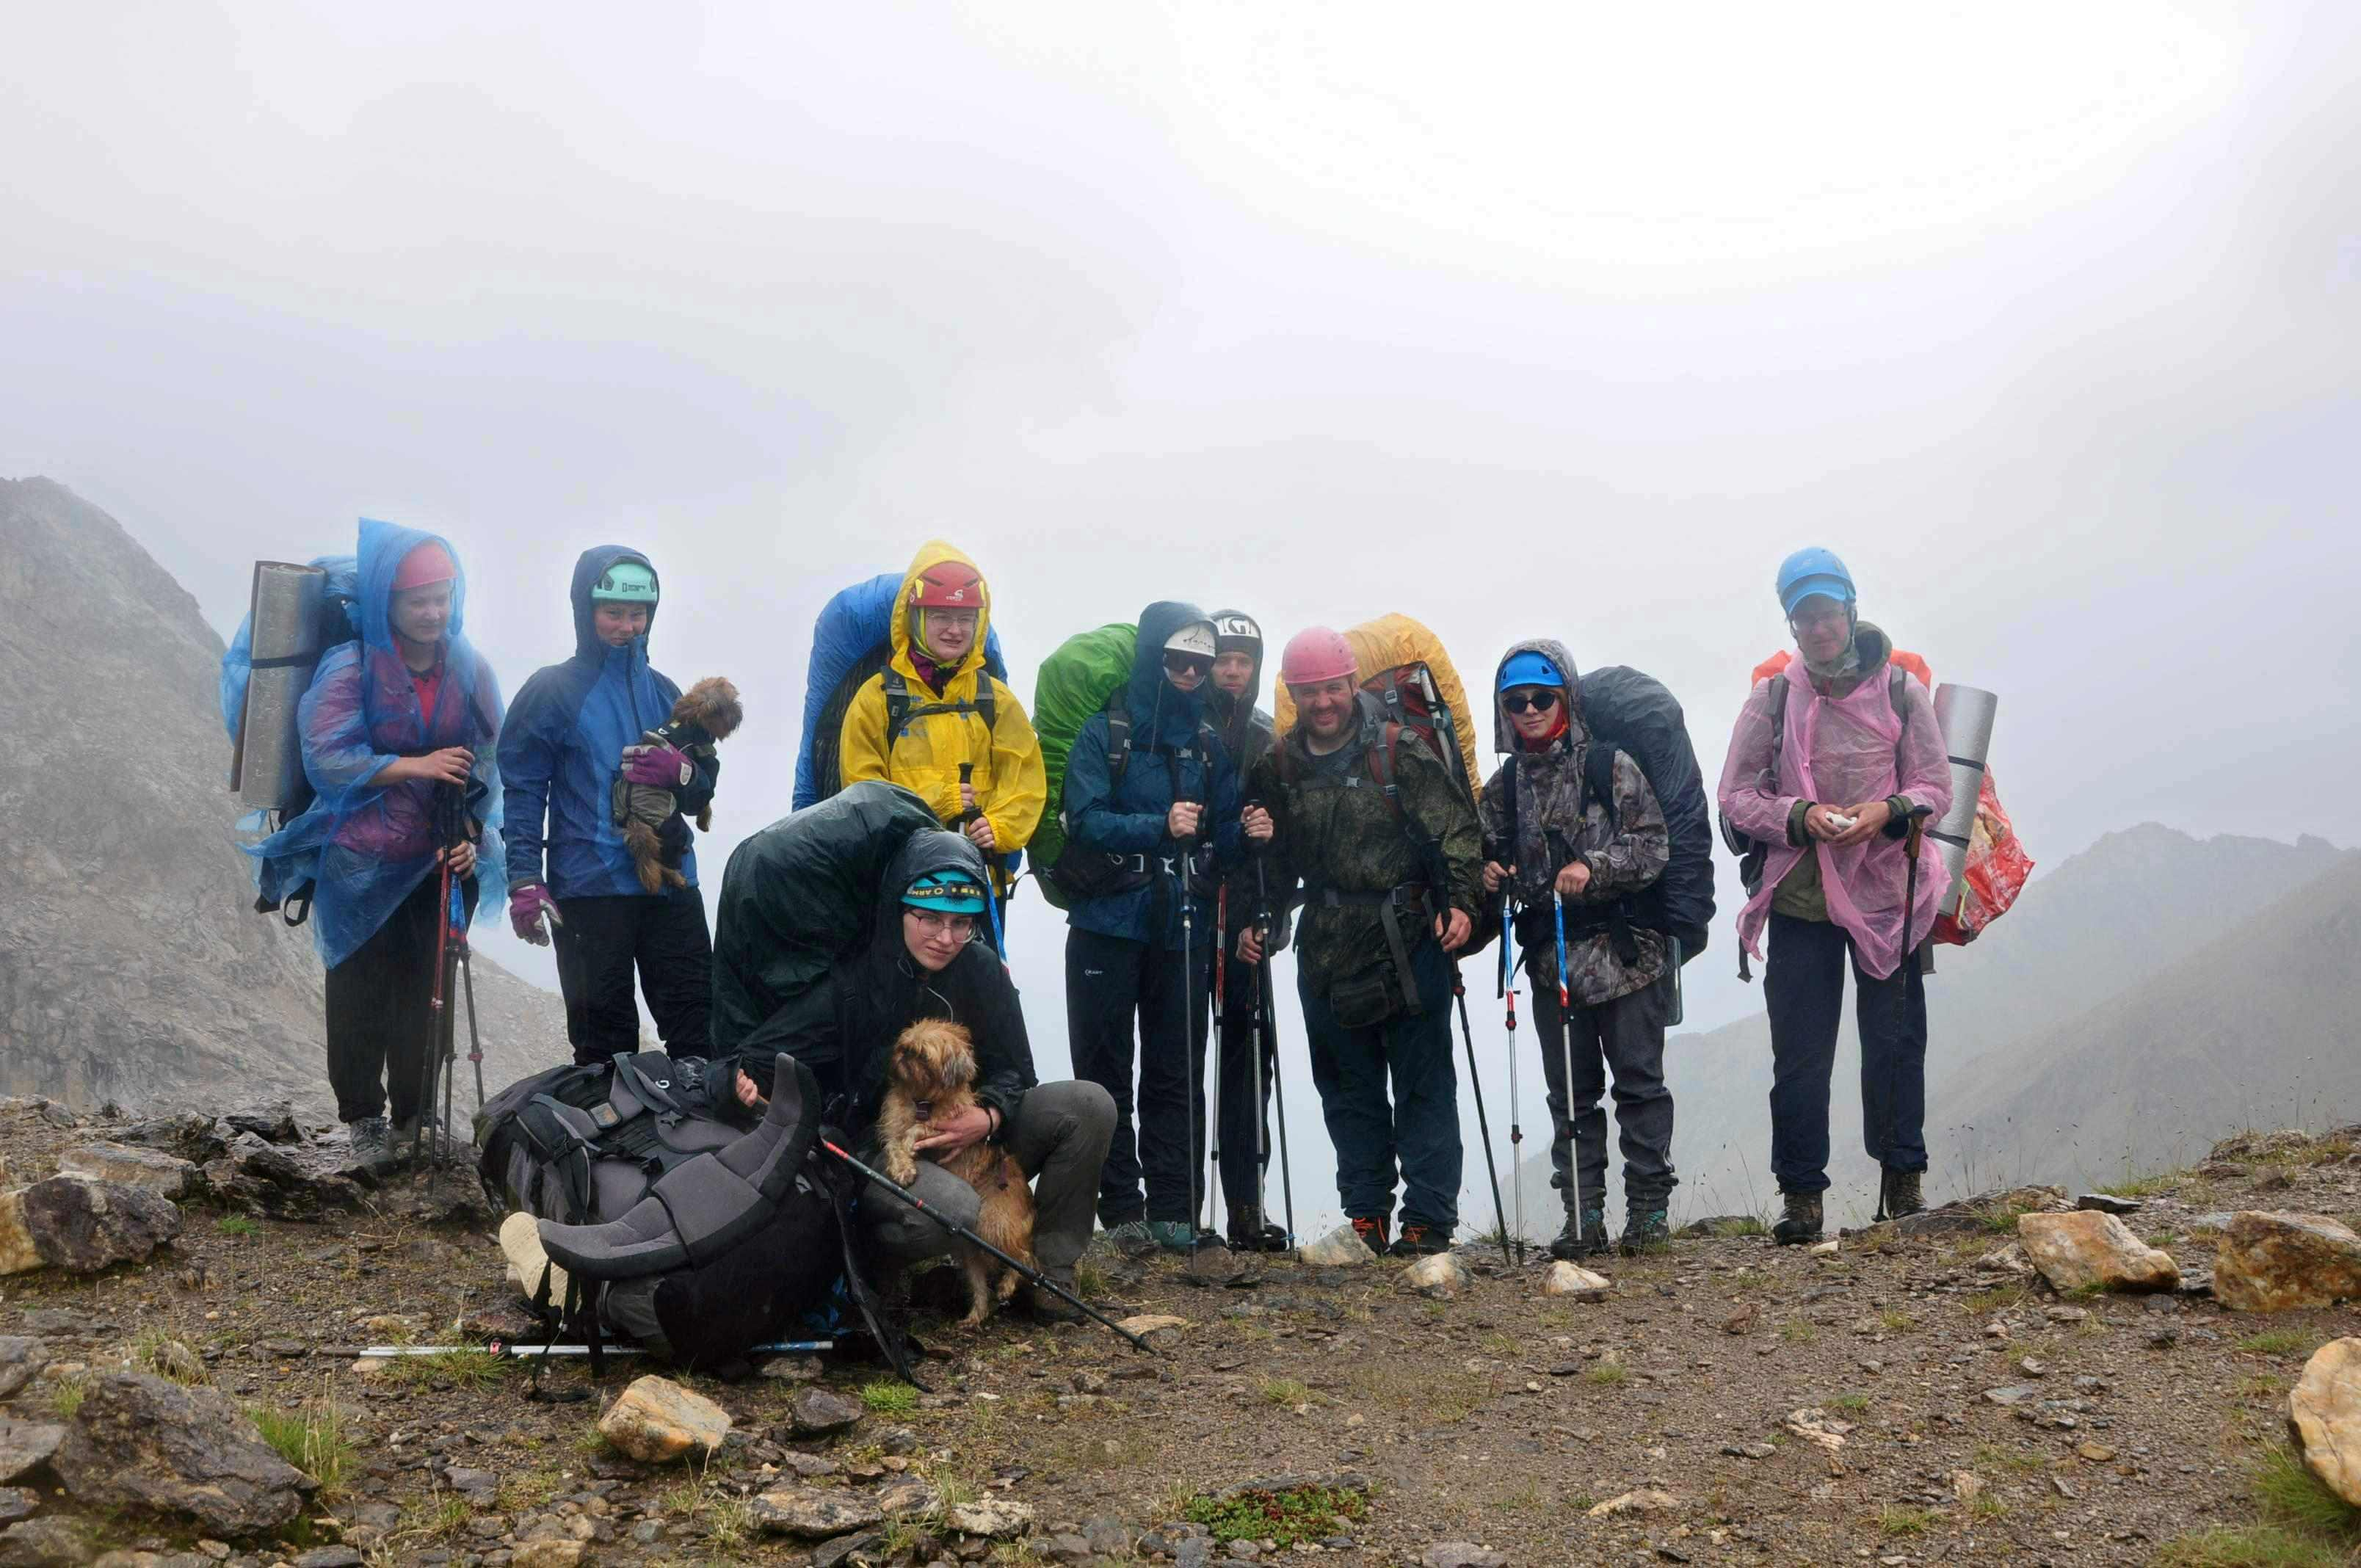
\includegraphics[width=0.99\linewidth]{../pics/DSC_0242.jpg}
	\end{minipage}
	\caption{Группа на пер. Кичкинекол Малый. Слева: вид в д.р. Чунгур-Джар, справа: вид в д.р. Таллычат}
	\label{fig:DSC_0239}
\end{figure}

Спуск идёт также по хорошо набитой тропе травянисто-осыпного склона. Идём по тропе, периодически встречаются туры, справа от тропы живописный вид на ГКХ, ледник Чунгур-Джар. Ливень превращается в мелкий дождь. В 15:00 спускаемся на урочище Аэродром в д.р Чунгур-Джар, на левом берегу находим огороженные камнями места под палатки и разбиваем лагерь. Дождь не прекращается, сопровождается сильным ветром.

Дежурные и руководитель готовят обед, остальные сушатся и греются в палатках. Координаты м.н. N43.248385\degree,~E42.236151\degree.

\begin{table}[h!]
	\centering
	\begin{tabular}{|c|c|c|c|c|c|} 
		\hline 
		Этап & ЧХВ \\ 	
		\hline 
		От а/л <<Узункол>> до начала косого траверса  & 01:05 \\
		Подъём косым траверсом из д.р. Кичкинекол до нижних ночёвок  & 01:18 \\
		Подъём к Поляне Крокусов & 01:00\\ 
		Подъём на седловину перевала & 02:08\\ 
		Спуск с седловины до урочища <<Аєродром>> & 01:07 \\
		
		\hline
		\textsc{Полное время подъёма на перевал  }& 05:38\\
		\textsc{Полное время спуска с перевала }& 01:07 \\
		\textsc{	Полное время прохождения перевала }& 06:45 \\
		\hline
	\end{tabular}
	\caption{Расклад времени, пер. Кичкинекол Малый}
\end{table}

\paragraph{Выводы и рекомендации:} ок

\clearpage